\section{Introdução}
\label{s.introduction}

\begin{frame}{Introdução}
	\vspace{0.4cm}
	\justify A área de Ciência da Computação sempre está evoluindo, onde diariamente dezenas de artigos novos estão disponíveis, e.g., \url{https://arxiv.org};
	\\~\\
	\begin{figure}
		\centering
		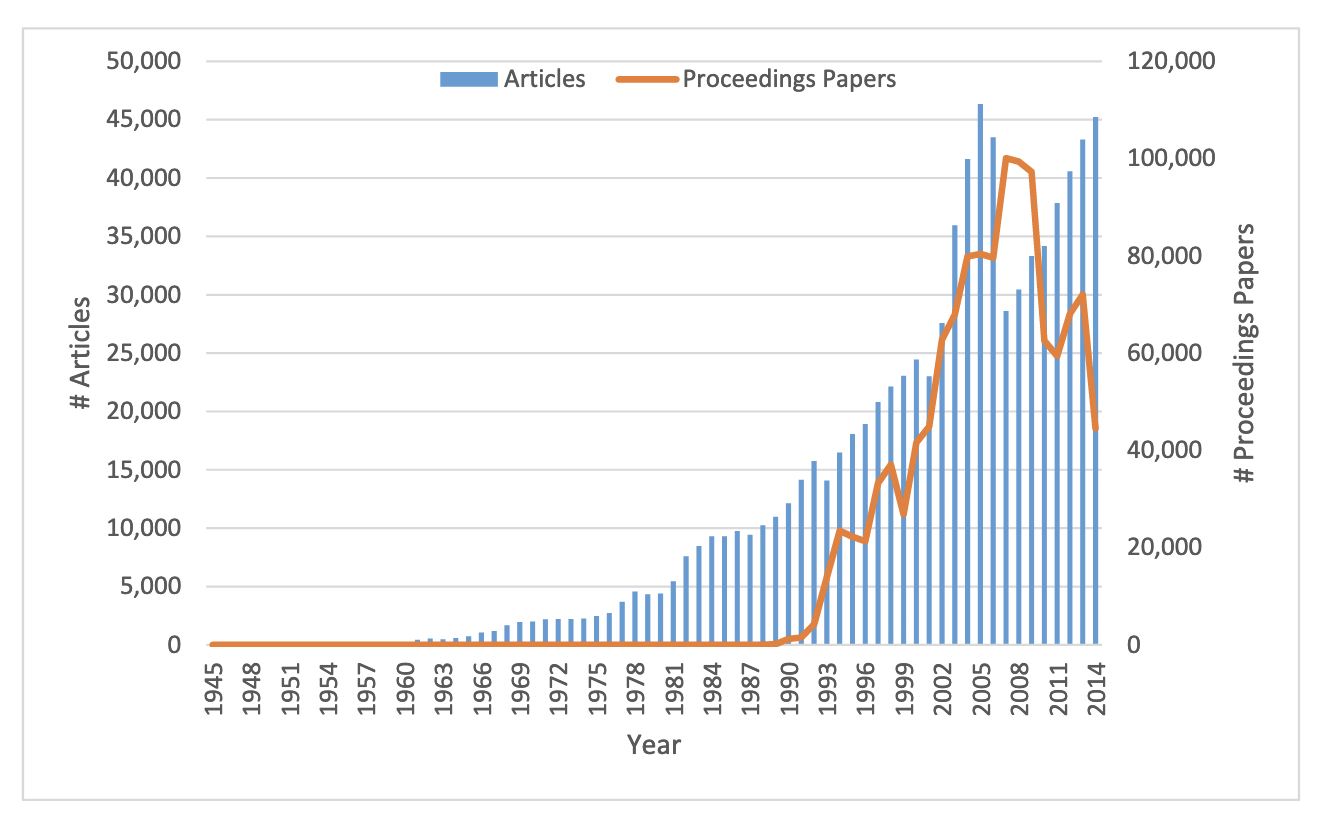
\includegraphics[scale=0.3]{figs/number_of_papers.png}
		\caption{Número de artigos (periódicos em azul e conferências em laranja) publicados em anos individuais~\cite{Fiala:17}.}
	\end{figure}
\end{frame}

\begin{frame}{}
	\begin{columns}
		\begin{column}{0.5\textwidth}
			\justify Atualmente, centros de pesquisa privados estão ``competindo"~diretamente com as universidades;	
		\end{column}
		\begin{column}{0.5\textwidth}
			\begin{figure}
				\centering
				
\includegraphics[scale=0.6]{figs/private_company.png}
			\end{figure}	
		\end{column}
	\end{columns}

\end{frame}

\begin{frame}{}
	\justify Entretanto, como é possível garantir a \textbf{visibilidade} da pesquisa em um mundo altamente competitivo?
\end{frame}